\documentclass[10pt,a4paper,twoside,onecolumn]{article}

% Use UTF-8 for plain tex files
\usepackage[utf8]{inputenc}

% Advanced math support
\usepackage{amsmath}

% Huge list of math symbols
\usepackage{MnSymbol}

% Set the margin from the page side
\usepackage[margin=3cm]{geometry}

% Support for internal links
\usepackage{hyperref}
\hypersetup{
    colorlinks=true,
    linkcolor=black,
    citecolor=black,
    filecolor=black,
    urlcolor=black,
}

% Leave out page numbers on empty pages
\let\origdoublepage\cleardoublepage
\renewcommand{\cleardoublepage}{%
  \clearpage
  {\pagestyle{empty}\origdoublepage}%
}

% Don't indent paragrpahs, instead separate them
\usepackage{parskip}
\setlength{\parskip}{5mm plus2mm minus3mm}
\setlength{\parindent}{0cm}

% Use alternative font (see http://www.tug.dk/FontCatalogue/ for alternatives)
\usepackage{cmbright}
\renewcommand*\familydefault{\sfdefault} % Set the default font to be sans-serif
\usepackage[T1]{fontenc}

% Set line height multiplicity
\linespread{1.05}

% Allow URL typesetting
\usepackage{url}

% Customize captions appearances 
\usepackage[margin=1cm]{caption}
\DeclareCaptionFormat{listing}{{\em #1#2#3}}
\captionsetup{
	format=listing,
	font={small},
}

% Enable advanced style specifications for the basic listing environments
% (enumerate, itemize, description)
\usepackage{enumitem}

% Customize headers and footers
\usepackage{fancyhdr}

% Includegraphics support
\usepackage{graphicx}

% Allows to change text color
\usepackage[usenames,dvipsnames,table<D-+>]{xcolor}

% Assign the LastPage label to the last page
\usepackage{lastpage}

% Enable the creation of appendices
\usepackage{appendix}

% Support for lists
\usepackage{etoolbox}
\usepackage{fp}

% Advanced templating support
\newcommand{\settitle}[2]{%
	\title{#1 -- #2}
	\def\doctitle{#1}
	\def\subtitle{#2}
}
\newcounter{mseaindex}
\newcounter{mseacount}
\newcommand{\addauthor}[1]{%
	\listadd{\authors}{#1}
	\stepcounter{mseacount}
}
\newcommand{\fmtauthor}[1]{#1}
\newcommand{\lineslist}[1]{#1\\}
\newcommand{\authorlines}{%
	\setcounter{mseaindex}{0}%
	\FPdiv{\limit}{\arabic{mseacount}}{2}%
	\FPround{\limit}{\limit}{0}%
	\renewcommand*{\do}[1]{%
		\ifnumequal{\value{mseaindex}}{0}{}{\ifnumequal{\value{mseaindex}}{\limit}{}{, }}%
		\ifnumequal{\value{mseaindex}}{\limit}{\\[0.7mm]\fmtauthor{##1}}{\fmtauthor{##1}}%
		\stepcounter{mseaindex}%
	}%
	\dolistloop{\authors}%
}

% Set layout lenghts
\setlength{\headheight}{8mm}
\setlength{\footskip}{1.5cm}
\addtolength{\textheight}{-.5cm}

% Set titles whitespace
\usepackage{titlesec}
\titlespacing{\section}{0mm}{8mm}{1mm}
\titlespacing{\subsection}{0mm}{3mm}{-2mm}
\titlespacing{\subsubsection}{0mm}{2mm}{-1mm}

% Enable code listings and set default options
\usepackage{listings}
\usepackage{courier} % Use Adobe Courier instead of Computer Modern Typewriter
                     % for monospaced text
\lstloadlanguages{python,bash,sh,xml}
\lstset{
	language=python,
	basicstyle=\footnotesize\ttfamily,
	stringstyle=\color{OliveGreen},
	numbers=left,
	numberstyle=\color{gray}\tiny,
	commentstyle=\color{magenta},
	keywordstyle=\color{MidnightBlue}\bfseries,
	frame=bt,
	rulecolor=\color{lightgray},
	numbersep=7pt,
	escapechar=!,
	extendedchars=true,
	captionpos=t,
	breaklines=true,
	showspaces=false,
	showtabs=false,
	tabsize=4, 
	xleftmargin=20pt,
	framexleftmargin=20pt,
	framexrightmargin=0pt,
	framexbottommargin=0pt,
	showstringspaces=false,
}

% Limit the TOC dept to sections and subsections
\setcounter{tocdepth}{2}

\usepackage{multirow} % Enable columns spawning multiple rows
\usepackage{tabularx}
\usepackage{booktabs} % Provides {top|middle|bottom}rule
\usepackage{longtable} % Support for tables spawning multiple pages,
                       % captions and footnotes.
                       % Does not work in multicolumn environments
% Define new tabularx column types:
%  - R: streteched right aligned
%  - C: stretched centered
\newcolumntype{R}{>{\raggedleft\arraybackslash}X}%
\newcolumntype{C}{>{\centering\arraybackslash}X}%
\renewcommand{\arraystretch}{1.3} % Set row height multiplicator
\usepackage{threeparttable} % Manual footnotes counter

% Provide support for (indented) unnumbered chapter and section titles
\usepackage{tocloft}
\newcommand{\uchapter}[1]{
	\chapter*{#1}
	\addcontentsline{toc}{chapter}{\hspace{\cftchapnumwidth}#1}
}
\newcommand{\usection}[1]{
	\section*{#1}
	\addcontentsline{toc}{section}{\hspace{\cftsecnumwidth}#1}
}

% Color definitions
\definecolor{highlightyellow}{RGB}{255,255,140}
\definecolor{mselogogray}{RGB}{96,101,109} % Color definition for the MSE logo

% Enable highlighting using \HighlightFrom and \HighlightTo
\usepackage{classes/highlighter}
\tikzset{highlighter/.style = {highlightyellow, line width = \baselineskip*.75}}
 


\settitle{Lab. 01 -- Port Scan}{Certified IT Security}
\addauthor{Julien Oberson}
\addauthor{Jonathan Stoppani}

\pagestyle{fancy}
\fancyhf{}
\renewcommand{\headrulewidth}{0pt}
\renewcommand{\footrulewidth}{0.6pt}

\fancyhead[LE]{%
	\raisebox{-0.15mm}{%
		
\includegraphics[height=6.3mm]{images/logo_mse_small}
		\hspace{5mm}\color{mselogogray}\rule[0mm]{0.5pt}{6mm}\hspace{4mm}}
	\begin{minipage}[b]{0.5\linewidth}
		\textcolor{mselogogray}{\uppercase{\scriptsize
			Certified IT Security\\[-1mm]
			Lab. 01 -- Port Scan}}
	\end{minipage}%
}

\fancyhead[RO]{%
	\begin{minipage}[b]{0.5\linewidth}
	\begin{flushright}
		\textcolor{mselogogray}{\uppercase{\scriptsize
			Julien Oberson\\[-1mm]
			Jonathan Stoppani}}
	\end{flushright}
	\end{minipage}
	\raisebox{-0.15mm}{%
		\hspace{4mm}\color{mselogogray}\rule[0mm]{0.5pt}{6mm}\hspace{5mm}
		
\includegraphics[height=6.3mm]{images/logo_mse_small}%
	}%
}

\fancyfoot[R]{\scriptsize\thepage\ of \pageref{LastPage}}
\fancyfoot[L]{\scriptsize\today}

\fancypagestyle{plain}{%
	\fancyhf{}
	\renewcommand{\footrulewidth}{0.6pt}
	\fancyfoot[R]{\scriptsize\thepage\ of \pageref{LastPage}}
	\fancyfoot[L]{\scriptsize\today}
}



\begin{document}

\title{Certified IT Secuirty\\  Lab. 01 -- Port scan}
\author{Julien Oberson \and Jonathan Stoppani}

\begin{titlepage}
\thispagestyle{empty}

\vspace*{10mm}

\includegraphics{images/logo_mse}
\vspace{5mm}

\hrule
\vspace{0.2mm}
{\Large Certified IT Security}\\[2mm]
{\Huge Lab. 01 -- Port scan}\\[1mm]
\hrule

\begin{minipage}[t]{0.5\textwidth}
    \begin{flushleft}
        Julien \textsc{Oberson}\\
        Jonathan \textsc{Stoppani}
    \end{flushleft}
\end{minipage}
\begin{minipage}[t]{0.495\textwidth}
	\begin{flushright}
        \today
	\end{flushright}
\end{minipage}

\vfill

\tableofcontents

\end{titlepage}


%\phantomsection
%\addcontentsline{toc}{chapter}{\hspace{\cftchapnumwidth}Contents}
%\pdfbookmark[0]{Contents}{toc:contents}
%\tableofcontents

\cleardoublepage
\setcounter{page}{1}

\section{Introduction}

The goal of this laboratory session is to execute a port scan of a given host (called \textit{server} from a remote machine (called \textit{client}) and to successively compare the results of this scan with a similar procedure executed locally on the targeted host.

During this laboratory session, we executed different measures by applying a different server setup for each round. The different setups, the results of the scanning sessions and an analysis of each scenario are presented in \autoref{sec:scans}.In the last section at the end of the present report, \autoref{sec:measurement}, we measure and quantify the overall security of the server using a formula allowing to empirically calculate an overall \textit{security factor} for a given host.

\subsection{Scan setup}

The \autoref{fig:measure-setup} below shows how the machines were wired together, their respective IP addresses at the moment of the scan and where each command was executed and with which target. As shown, the setup is very simply and consists of only two machines (a client: 160.98.21.145 and a server: 160.98.21.224) connected over a simple Ethernet link.

\begin{figure}[ht]
	\centering
	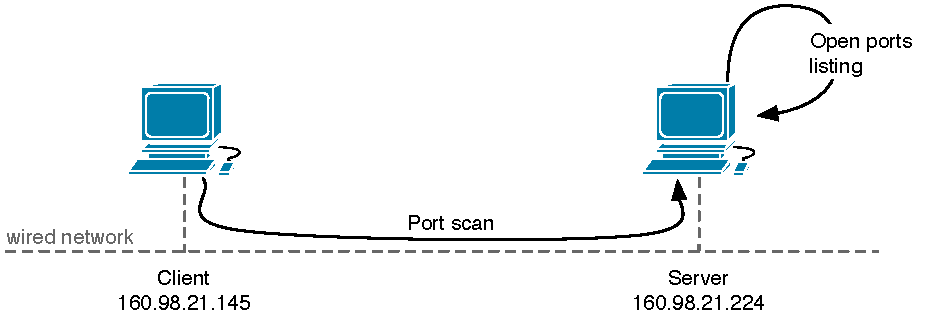
\includegraphics[width=0.9\textwidth]{images/measure-setup}
	\caption{Scan and measurement setup}
	\label{fig:measure-setup}
\end{figure}

As already anticipated, the port scan was executed from the client by setting the server as target, while the listing of open ports was executed directly on the target.

\subsection{Commands}

Mainly two commands were used to execute the different port scannings and listings. Hereafter we introduce them generally, while for each measure---presented in the following section---we include the exact command which was used to obtain the given result.

Additional tools (i.e. wireshark, \texttt{ping}, \texttt{ssh},...) where also used in order to setup the measurement environment or to gather a better overall understanding of the exact operation mode of the two main commands we employed, but---as they belong to the basic toolkit of every IT engineer---are not described here.

\subsubsection{\texttt{nmap}}

We used this first tool, called \texttt{nmap}, to execute the port scans on the remote host. The \texttt{nmap} man page describes it as follows:

\begin{quote}
	Nmap ("Network Mapper") is an open source tool for network exploration and security auditing.
	Itwas designed to rapidly scan large networks, although it works fine against single hosts.
	Nmap uses raw IP packets in novel ways to determine what hosts are available on the network, what services (application name and version) those hosts are offering, what operating systems (and OS versions) they are running, what type of packet filters/firewalls are in use, and dozens of other characteristics.
\end{quote}

For the different scan sessions, we took advantage of some of the options which this command takes, as explained hereafter. For a full options listing refer to the man page itself.

% Used commands:
% nmap -sV -PN 160.98.21.224
% nmap -sU -PN 160.98.21.224
% nmap -sU -PN -p 1-1024 160.98.21.224
% nmap -sU -PN -p 1-1024 160.98.21.224
% nmap -sU -PN -p 1-1024 160.98.21.224

\begin{description}[style=multiline,leftmargin=1cm]
	\item[\texttt{-p}] This option allows to specify one or more port ranges to be tested. It allows also to specify if the range refers to UDP ports or TCP ports by using a prefix (\texttt{U:} and \texttt{T:}, respectively).
	\item[\texttt{-PN}] Treats all hosts as online and skips host discovery. Discovery of online hosts is normally used when instructing \texttt{nmap} to scan a huge list of IPs or using address patterns and we don't know which ones are online.
	\item[\texttt{-sU}] Performs a UDP ports scan by sending a packet to each targeted port and waiting for either a UDP response or an ICMP message from the remote host. UDP scanning is slow because if a port is open or filtered, \texttt{nmap} has to timeout before marking it as \texttt{open|filtered}.
	\item[\texttt{-sV}] Probes open ports to determine service/version info by using the \texttt{nmap-services} database which contains about 2200 well-known service probes to send appropriate requests and fingerprints to parse the obtained responses.
\end{description}

\subsubsection{\texttt{lsof}}
\label{sec:lsof}

The \texttt{lsof} command can be used to list information about files opened by processes running on the \emph{local} system. As on unix \emph{everything is a file}, processes listening on ports have to open a socket in order to do so and are thus also listed.

By combining the \texttt{lsof} command with some specific options and filtering the output using \texttt{grep}, it is possible to obtain the exact list of open ports on each interface of the host. The full command line used to capture this list is given in \autoref{lst:lsof}.

\lstset{language=bash,caption=Complete shell command to list open ports,label=lst:lsof,numbers=none}
\begin{lstlisting}
sudo lsof -i -n -P | grep LISTEN | grep -v -E '127.0.0.1|\[::1\]'
\end{lstlisting}

The use of \texttt{sudo} is needed to list all processes, including those run by \texttt{root} or by other users on the system, while the filtering over the \texttt{LISTEN} keyword is needed in order to avoid listing descriptors belonging to connections in different states (i.e. \texttt{ESTABLISHED}, \texttt{CLOSED},...). Additionally, we filter out all services listening only on the loopback interface (either IPv4 or IPv6) with the second \texttt{grep} round.

The different options used for the \texttt{lsof} command have the following semantics:

\begin{description}[style=multiline,leftmargin=*]
	\item[\texttt{-i}] This options limit the listing of all Internet and x.25 network files. If an optional address is given, the listing will be limited to that specific interface. Additionally, the flags \texttt{-i4} and \texttt{-i6} allow to limit the listing to IPv4 or IPv6 connections, respectively.
	\item[\texttt{-n}] This options simply disables reverse DNS lookups for each network number (normally an IP address) for network files. It also makes \texttt{lsof} run much faster.
	\item[\texttt{-P}] This options is the same as the \texttt{-n} option but disables the conversion of port number to service names.
\end{description}

\section{Port scans and listings}
\label{sec:scans}

After the first, straight port scan, we decided to modify the configuration of the and to prove that the changes are reflected in the port scan as well. In order to do so, we created different configuration sets and executed a port scan session for each one. These different configuration sets and the respective results are illustrated in the following subsections.

\subsection{Basic TCP port scan}
\label{sec:basic}

As first operation, we issued a complete port scan from the client toward the remote host. We explicitly set the port range in order to scan all ports (from 1 to 65535). Once the scan was done, we listed the different processes active on the target using the \texttt{lsof} command introduced in the \autoref{sec:lsof}.

The \autoref{lst:tcp-plain} shows the results of the execution of the \texttt{nmap} command (the complete synopsys is reported in the \autoref{lst:nmap-plain}), while the \autoref{lst:lsof-plain} shows the results of the execution of the \texttt{lsof} command.

\lstset{language=bash,caption=Complete \texttt{nmap} invocation for a TCP scan,label=lst:nmap-plain,numbers=none}
\begin{lstlisting}
nmap -PN -p 1-65535 160.98.21.224
\end{lstlisting}

\lstset{language=,caption=Output of the \texttt{nmap} execution for a TCP scan,label=lst:tcp-plain}
\begin{lstlisting}
Starting Nmap 5.21 ( http://nmap.org ) at 2012-02-20 13:01 CET
Nmap scan report for Culhaven.sofr.hefr.lan (160.98.21.224)
Host is up (0.00075s latency).
Not shown: 65526 closed ports
PORT      STATE    SERVICE
22/tcp    open     ssh
80/tcp    open     http
548/tcp   open     afp
631/tcp   open     ipp
5900/tcp  open     vnc
10631/tcp open     unknown
17500/tcp open     unknown
23053/tcp open     unknown
49152/tcp open     unknown

Nmap done: 1 IP address (1 host up) scanned in 674.50 seconds
\end{lstlisting}

\lstset{caption=Output of the \texttt{lsof} execution to list TCP sockets,label=lst:lsof-plain}
\begin{lstlisting}
launchd       1      root  IPv4  TCP *:5900 (LISTEN)
launchd       1      root  IPv6  TCP *:5900 (LISTEN)
launchd       1      root  IPv4  TCP *:548 (LISTEN)
launchd       1      root  IPv6  TCP *:548 (LISTEN)
launchd       1      root  IPv4  TCP *:22 (LISTEN)
launchd       1      root  IPv6  TCP *:22 (LISTEN)
ODSAgent     64      root  IPv6  TCP *:49152 (LISTEN)
kdc          73      root  IPv6  TCP *:88 (LISTEN)
Printopia   500  garetjax  IPv6  TCP *:10631 (LISTEN)
Growl       504  garetjax  IPv4  TCP *:23053 (LISTEN)
Growl       504  garetjax  IPv6  TCP *:23053 (LISTEN)
Dropbox    9474  garetjax  IPv4  TCP *:17500 (LISTEN)
cupsd     19289      root  IPv4  TCP *:631 (LISTEN)
cupsd     19289      root  IPv6  TCP *:631 (LISTEN)
named     20543      root  IPv4  TCP 192.168.2.1:53 (LISTEN)
httpd     20561      root  IPv6  TCP *:80 (LISTEN)
httpd     20563      _www  IPv6  TCP *:80 (LISTEN)
httpd     20988      _www  IPv6  TCP *:80 (LISTEN)
\end{lstlisting}

If we compare the two listings, we notice straight away that \texttt{nmap} didn't detect open IPv6 ports; in fact, IPv6 port scan has to explicitly be enabled using the \texttt{-6} flag and by providing a valid IPv6 address. Apart from this first difference, if we analyze the two listings in more depth, we can conclude that \texttt{nmap} was able to find all open ports except for the \texttt{named} process, listening on \texttt{192.168.2.1:53}. This is due to the fact that we executed the scan towards the interface with the IP address 160.98.21.224 and are thus enable to reach services listening on a different interface.

From this first measurements round, we learnt that a simple port scan using \texttt{nmap} is not enough to determine the exposure of a system, as the system can run vulnerable services running on different interfaces which may be accessible too. Additionally, two scans have to be performed, once for IPv4 and once for IPv6 as an attacker could chose to use either version.

To conclude we can say that---if we have access to the target---it is always better to list the open directly ports using \texttt{lsof}. This method also has the added value of displaying the process and the user to which the socket belongs to.

\subsection{Disabling services}

After the first scan report, we tried to disable the different services and try to reduce the number of open ports in order to have a more secure system. We began by identifying the services we can stop using the output of the \texttt{lsof} command issued in the last session.

As the target host runs OS X, most of these services can be deactivated from the system preferences, as shown in the \autoref{fig:sysprefs}. The new settings did shutdown the following services: ssh (\emph{Remote Login}), http (\emph{Web Sharing}), afp (\emph{File Sharing}), ipp (\emph{Printer Sharing}, \emph{Scanner Sharing}), vnc (\emph{Screen Sharing}). Additionally, the \texttt{names} process---previously listening on 192.168.2.1:53---was also shutdown by disabling \emph{Internet Sharing}.

\begin{figure}[ht]
	\centering
	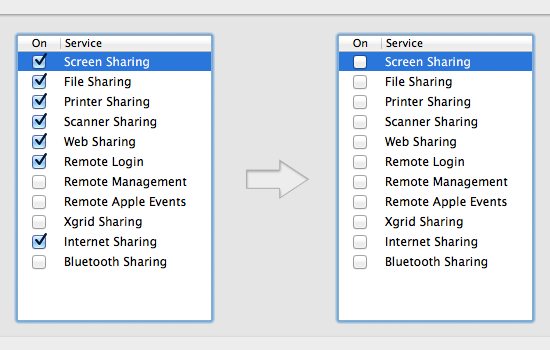
\includegraphics[width=0.6\textwidth]{images/sysprefs}
	\caption{Disabling services from the system preferences}
	\label{fig:sysprefs}
\end{figure}

We also stopped the remaining processes belonging to the \texttt{root} user, namely the \texttt{ODSAgent}\footnote{The \texttt{ODSAgent} process is responsible to manage Apple's \emph{CD \& DVD Sharing} feature which can be disabled in the system preferences. In our case, the option doesn't show up because the host doesn't have a CD-ROM drive. We can disable the daemon by executing \texttt{sudo launchctl unload -w /System/Library/LaunchDaemons/com.apple.ODSAgent.plist}}
and the \texttt{kdc}\footnote{\texttt{kdc} is used for single sign-on features on a Mac OS X Server network; once all file sharing features are disabled, the \texttt{kdc} daemon has no more reason to run and can also be stopped: \texttt{sudo launchctl unload -w /System/Library/LaunchDaemons/com.apple.Kerberos.kdc.plist}}
and the four unknown services listening on unprivileged ports belonging to the user \texttt{garetjax}: \emph{Printopia}, \emph{Growl} and \emph{Dropbox}.

After having shutdown all services and applications, we relaunched \texttt{lsof} and obtained en empty result. This indicates that there isn't any process which currently listens on a TCP port on the target. This result is coherent with an additional port scan that also returned no results, as shown in the \autoref{lst:tcp-strict}.

\lstset{language=,caption=Output of \texttt{nmap} with some services disabled,label=lst:tcp-strict}
\begin{lstlisting}
Starting Nmap 5.21 ( http://nmap.org ) at 2012-02-20 13:01 CET
Nmap scan report for Culhaven.sofr.hefr.lan (160.98.21.224)
Host is up (0.00075s latency).
All 65535 scanned ports on 160.98.21.224 are closed.

Nmap done: 1 IP address (1 host up) scanned in 665.09 seconds
\end{lstlisting}

\subsection{Basic UDP port scan}

In the previous subsections, we have discusssed the results for a TCP port scan for different configurations. In the present and the following subsections, we would like to analyze the results of a UDP port scan on the same setup. As we did for the TCP scan, let's begin with a simple UDP port scan. In this case, we limit the port range to the ports between 1 and 1024, in order to speedup the overall execution while maintaining a reasonable probe timeout.

Instead of launching a well-known UDP service on the target, we created our custom server and set it to listen on the port 1024. This allows us to chose exactly what to do when the UDP probe is received and to have a real-time feedback of the event. In our case, the server was configured to simply print out the reception of the probe sent by \texttt{nmap}\footnote{The code of the server and the usage instructions are provided in the Appendix~\ref{sec:udp-server} at the end of the present report.}.

The exact \texttt{nmap} command used to launch the port scan is shown in the \autoref{lst:nmap-udp} below. In this case, we made some modifications to the invocation: to perform an UDP scan, it is necessary to have administrator privileges on the client machine (hence the use of \texttt{sudo}), additionally, to raise the confidence not to miss any probe reply, we set the timing template to \texttt{sneaky}\footnote{Timing templates regulate different parameters bound to concurrency, rates, retransmission limits, timeout,... The \texttt{sneaky} template sends UDP probes without any parallelism and at an interval of 0.4s} using the \texttt{-T2} flag.
\lstset{language=bash,caption=Complete \texttt{nmap} invocation to scan UDP ports,label=lst:nmap-udp,numbers=none}
\begin{lstlisting}
sudo nmap -sU -p 1-1024 -T2 160.98.21.224
\end{lstlisting}

The \texttt{lsof} invocation has also to be updated to list open UDP sockets; the modifications are reported in the \autoref{lst:lsof-udp}. In this case, we can specify the UDP filter directly as an argument to the \texttt{-i} option and we have to remove the \texttt{LISTEN} filter.

\lstset{language=bash,caption=Complete \texttt{lsof} invocation to list UDP sockets,label=lst:lsof-udp,numbers=none}
\begin{lstlisting}
sudo lsof -i udp -n -P | grep -v -E '127.0.0.1|\[::1\]|\*:\*'
\end{lstlisting}

The results of the invocation of these two commands are shown in the \autoref{lst:udp-plain} and \autoref{lst:lsof-udp-plain} below, respectively (custom UDP server port and process lines are highlighted).

\lstset{language=,caption=Output of the \texttt{nmap} execution for a UDP scan,label=lst:udp-plain}
\begin{lstlisting}
Starting Nmap 5.21 ( http://nmap.org ) at 2012-02-20 13:01 CET
Nmap scan report for Culhaven.sofr.hefr.lan (160.98.21.224)
Not shown: 1020 closed ports
PORT     STATE         SERVICE
123/udp  open          ntp
137/udp  open|filtered netbios-ns
138/udp  open|filtered netbios-dgm
!\HighlightFrom!1024/udp open|filtered unknown!\HighlightTo!

Nmap done: 1 IP address (1 host up) scanned in 416.98 seconds
\end{lstlisting}

\lstset{caption=Output of the \texttt{lsof} execution to list UDP sockets,label=lst:lsof-udp-plain}
\begin{lstlisting}
launchd       1      root  IPv4  UDP *:137
launchd       1      root  IPv4  UDP *:138
ntpd         52      root  IPv4  UDP *:123
ntpd         52      root  IPv6  UDP *:123
ntpd         52      root  IPv6  UDP [fe80:1::1]:123
ntpd         52      root  IPv6  UDP [fe80:5::fa1e:dfff:fedf:57c3]:123
ntpd         52      root  IPv4  UDP 169.98.21.224:123
netbiosd    186  _netbios  IPv4  UDP *:138
netbiosd    186  _netbios  IPv4  UDP *:137
!\HighlightFrom!python    34313  garetjax  IPv4  UDP *:1024!\HighlightTo!
\end{lstlisting}

Additionally, the custom UDP server confirms that the UDP probe was received, as shown in the \autoref{lst:udp-out} below.

\lstset{caption=Output of the custom UDP server during the port scan,label=lst:udp-out}
\begin{lstlisting}
received '' from 160.98.21.145:37576
received '' from 160.98.21.145:37577
\end{lstlisting}

In this port scan session, \texttt{nmap} reported that---in the 1-1024 range---there were 1020 closed ports, 3 open or filtered and one surely open. How was \texttt{nmap} able to define these states? The \autoref{fig:wireshark} shows an extract of the measure we run with \emph{Wireshark} while executing the scan and allows to precisely define what happened.

\texttt{nmap} sends a UDP datagram, called \emph{probe} to each port it has to test (as shown in the \emph{Wireshark} measure by the number 1) and then waits for a reply. The \texttt{ntp} port was determined to be open because the client received a UDP reply (as shown in the figure by the numer 2). Similarly, it was possible to determine that 1020 ports were closed because the server sent back an ICMP message \texttt{Destination unreachable (Port unreachable)} for each probe sent to them (number 3). The state of the remaining three ports could not be determined for sure, because neither a reply nor an ICMP message was received and was thus set to \texttt{open|filtered}.\footnote{In this case, the three filtered ports are probably open, as for the remaining 1020 ports, an ICMP message was correctly received.}

\begin{figure}[ht]
	\centering
	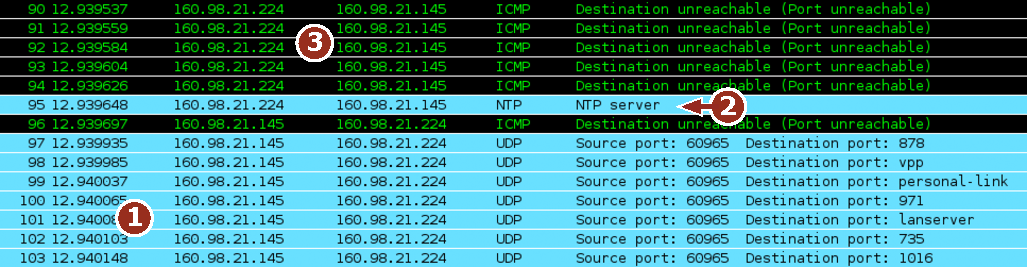
\includegraphics[width=1\textwidth]{images/wireshark}
	\caption{Wireshark measure of the UDP port scan}
	\label{fig:wireshark}
\end{figure}


\subsection{Stealth mode UDP scan}

Mac OS X has a special firewall mode called "Stealth Mode". Depsite his name, this mode simply blocks all ICMP traffic which could leak information about the state of the host: this means mainly no more \texttt{Echo reply} and \texttt{Destination unreachable} messages.

We supposed that we the firewall is configured in this mode, all ports but the one which was previously listed as \texttt{open} should now be listed in the \texttt{open|filterd} mode as \texttt{nmap} is no more able to determine their state. This supposition was confirmed by an additional \texttt{nmap} round, as shown in the \autoref{lst:nmap-stealth}.

\lstset{caption=Output of the custom UDP server during the port scan,label=lst:nmap-stealth}
\begin{lstlisting}
Starting Nmap 5.21 ( http://nmap.org ) at 2012-02-20 13:15 CET
Nmap scan report for Culhaven.sofr.hefr.lan (160.98.21.224)
Host is up (0.00092s latency).
!\HighlightFrom!Not shown: 1023 open|filtered ports!\HighlightTo!
PORT    STATE SERVICE
137/udp open  netbios-ns

Nmap done: 1 IP address (1 host up) scanned in 19.15 seconds
\end{lstlisting}

\section{Security measurement}
\label{sec:measurement}

As a last task for this lab, it was asked to find a measure for the level of security offered by the tested server. We define the security level for the original configuration of the server, e.g. as applied in the first port scan in \autoref{sec:basic}.

To define a security measurement, we intended to use a simplified version of RAV (Risk Assessment Value) method, based on the data we know. In our case, we can take into account the following three aspects (the definitions are taken from the \emph{Open Source Security Testing Methodology Manual}):

\begin{description}
	\item[Operational Security, Access] is calculated by the number of different places where the interaction can occur. Removing direct interaction with an asset will halve the number of ways it can be taken away.
	\item[Actual Security, Vulnerability] is the flaw or error that: (a) denies access to assets for authorized people or processes, (b) allows for privileged access to assets to unauthorized people or processes, or (c) allows unauthorized people or processes to hide assets or themselves within the scope.
	\item[Exposure] is an unjustifiable action, flaw, or error that provides direct or indirect visibility of targets or assets within the chosen scope channel.
\end{description}

However, producing an actual score based on this three aspects only (out of the 18 presented in the complete RAV calculation) is not possible.

Translated for our setup and use case, these three aspects can be defined as follows:

\begin{description}
	\item[Operational Security, Access] is calculated by the number of open TCP or UDP ports on the target system. This value can directly be deferred from the port scan results presented earlier in this report.
	\item[Actual Security, Vulnerability] is calculated using the number and severity of the know bugs found in the processes previously found listening on TCP or UDP ports. This value can be calculated by looking up a bugs database once the versions of the different services is known.
	\item[Exposure] is calculated by the number of processes listening on TCP or UDP ports and which have not a well defined goal in the current target operation mode. This value can be defined by first deciding if a process is needed or not to reach the goal for which the host is operating.
\end{description}

\subsection{Access}

The \autoref{tab:report} summarizes all the open ports found by the first scan and adds the information about service versions as discussed in the next subsection. By a rapid overview of the table, there is a total of 10 open ports; we will use this number later to try to measure the security level of this host.

\begin{table}
\begin{threeparttable}[b]
\begin{tabularx}{\textwidth}{ c c | l l | l X }

\toprule

% Headers
\multirow{2}{*}{Proto.} &
\multirow{2}{*}{Port} &
\multicolumn{2}{c|}{\texttt{nmap} detection} &
\multicolumn{2}{c}{Local inspection} \\
\cline{3-6} & &
\multicolumn{1}{c}{Service} &
\multicolumn{1}{c|}{Version} &
\multicolumn{1}{c}{Process} &
\multicolumn{1}{c}{Version} \\
\hline

% Contents
TCP & 22 & ssh & OpenSSH 5.6 & sshd & OpenSSH 5.6p1, OpenSSL 0.9.8r \\
TCP & 80 & http & Apache 2.2.21\tnote{1} & httpd & 2.2.21 (Unix) \\
TCP & 548 & afp & -- & afp & n/d\tnote{2} \\
TCP & 631 & ipp & CUPS 1.5 & cupsd & 1.5.1 \\
TCP & 10631 & unknown & -- & Printopia & 2.0  \\
TCP & 17500 & unknown & -- & Dropbox & 1.2.52 \\
TCP & 23053 & tcpwrapped & -- & Growl & 1.3.3 \\
UDP & 123 & ntp & NTP v4 & ntpd & 4.2.6 \\
UDP & 137 & netbios-ns & -- & netbiosd & n/d\tnote{2} \\
UDP & 138 & netbios-dgm & -- & netbiosd & n/d\tnote{2} \\

\bottomrule
\end{tabularx}

\begin{tablenotes}
	\item[1] Full service ID: \texttt{Apache httpd 2.2.21 ((Unix) mod\_ssl/2.2.21 OpenSSL/0.9.8r DAV/2 PHP/5.3.8 with Suhosin-Patch)}
	\item[2] These services are provided by proprietary OS packages and their version is bundled to the version of the specific OS version.
\end{tablenotes}

\caption{Summary of open ports, service information as detected by \texttt{nmap} and processes found by locally inspecting the target}
\label{tab:report}
\end{threeparttable}
\end{table}


\subsection{Vulnerability}

As anticipated in the previous subsection, the \autoref{tab:report} also contains running services and their versions. This data is retrieved using the \texttt{nmap} service discovery capability and by locally inspecting the target for the actual services and their versions. The full command line used to detect service/version info through \texttt{nmap} is reported in the \autoref{lst:nmap-versions}.

\lstset{caption=Command to execute service detection on the previously found open ports,label=lst:nmap-versions}
\begin{lstlisting}
sudo nmap -sV -sU -sS -p 22,80,123,137,138,548,631,10631,17500,23053 160.98.21.224
\end{lstlisting}

\begin{table}
\begin{center}
\begin{threeparttable}[b]
\begin{tabularx}{0.75\textwidth}{ X | c | c | c }

\toprule

% Headers
Service & Known vuln.\tnote{1,2} & Max. Criticity\tnote{1} & Never version available \\

\hline

% Contents
sshd\tnote{3} & 4 + 8 & 7.5, 9.3 & Yes (5.9p1, 1.0.0g) \\ %http://web.nvd.nist.gov/view/vuln/search-results?query=OpenSSH&search_type=last3years&cves=on
httpd & 2 & 4.3 & Yes (2.4.1)  \\ %http://web.nvd.nist.gov/view/vuln/search-results?page_num=0&cves=true&query=httpd+apache&pub_start_date=02-2009&pub_end_date=02-2012&uscert_ta=false&uscert_vn=false&oval_query=false&adv_search=false
afp & 0 & -- & No \\ % http://web.nvd.nist.gov/view/vuln/search-results?query=afp&search_type=all&cves=on
cupsd & 0 & -- & Yes (1.5.2) \\ % http://web.nvd.nist.gov/view/vuln/search-results?query=cups&search_type=all&cves=on
Printopia & 0 & -- & Yes (2.1.5) \\
Dropbox & 0 & -- & No \\
Growl & 0 & -- & No \\
ntpd & 0 & -- & No \\
netbiosd & 0 & -- & No \\

\bottomrule
\end{tabularx}

\begin{tablenotes}
	\item[1] The list of vulnerabilities and their criticity was retrieved from the National Vulnerability Database of the USA: \url{http://nvd.nist.gov/}
	\item[2] This number refers only to the known vulnerabilities listed on the NVD website. Other resources are available but weren't consulted.
	\item[3] Numbers refer to the version of OpenSSH and OpenSSL, respectively.
\end{tablenotes}


\caption{Summary of known vulnerabilities in the detected versions of the running software and their patching state.}
\label{tab:bugs}
\end{threeparttable}
\end{center}
\end{table}

The \autoref{tab:bugs} lists the number of known bugs alongside with their maximal criticity, as well as the upgrade potential for the different versions of the software running on the target.


\subsection{Exposure}

The definition of exposure for the inspected target highly depends on its usage: if it is used as a simple webserver, the majority of the processes (i.e. \texttt{afp}, \texttt{cupsd}, \texttt{Printopia},...) should not be running; if instead it is used as a personal desktop, then the execution of these softwares is justified.

In this case, we consider the machine as a generic server providing services such as file sharing, printing and web hosting to the users of a network. In this case, the following softwares have no reason to be running: \texttt{Printopia}, \texttt{Dropbox} and \texttt{Growl}.

\subsection{Risk Assessment Value}

Our audit is over-simplistic and the collected data does not suffice to calculate a reliable RAV, we tried to apply the model just the same but having only 3 factors at our disposal made the task too difficult. We invented thus our own measurement scale based on the following "per port" factors:

\vspace{-.5cm}
\begin{align*}
	N_{vuln} &= \text{Number of vulnerabilities (minimum value: 1)} \\
	 C_{max} &= \text{Max criticity (minimum value: 1)} \\
  E_{factor} &= \left\{
		\begin{array}{l l}
			1 & \quad \text{if the service has a reason to run}\\
		   10 & \quad \text{if the service has no reason to run}\\
		\end{array}
	\right.
\end{align*}

The overall security grade is then calculated as shown in \autoref{eq:fact} and \ref{eq:sec}. This function results in an exponentially decreasing curve, as represented in the \autoref{fig:sec-plot}.

\vspace{-.5cm}
\begin{align}
	\label{eq:fact}
Factor &= \sum\limits^{ports}{N_{vuln} \cdot E_{factor} \cdot {C_{max}}^2}\\
	\label{eq:sec}
   Security &= \exp\left(-{Factor \over 75}\right)
\end{align}

\begin{figure}[ht]
	\centering
	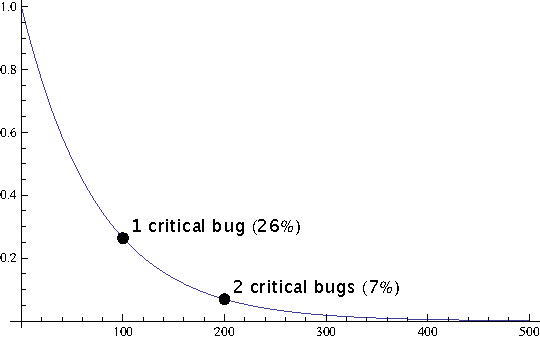
\includegraphics[width=.6\textwidth]{images/sec-plot}
	\caption{Security function, including the resulting security percentage for a system with one, respectively two, severe security flaws}
	\label{fig:sec-plot}
\end{figure}

Based on the measurements and considerations expressed in the previous sub sections, we can calculate the $Security$ value for the target host by applying the formulas \ref{eq:fact} and \ref{eq:sec} as shown in the \autoref{eq:sec-sys}.

\vspace{-.5cm}
\begin{align}
	Factor &= 12 \cdot 1 \cdot 9.3^2 + 2 \cdot 1 \cdot 4.3^2 + 1 + 1 + 10 + 10 + 10 + 1 + 1 \nonumber\\
			 &= 1037.88 + 36.98 + 34 \nonumber\\
			 &= 1108.86\nonumber\\
	\label{eq:sec-sys}
	Security &= \exp\left(-{1108.96\over75}\right) = 3.788 \times 10^{-7} = 0.00004\%
\end{align}

The resulting security grade is extremely low, but considering on one side the high number of security flaws in the \texttt{ssh} package and, on the other side, the simplicity of our empirically crafted formula, such a value is expected.

In order to provide a more statistically correct and reliable result, many additional security aspects of the examined systems have to be audited. This was however out of the scope of this laboratory and will probably be the subject of the next sessions and was thus temporarily left aside.

\section{Conclusions}

In this report, we explained how to scan a host using the \texttt{nmap} program, how to analyze the results and how to compare them with a local process listing.

While the TCP scans gave stable results, UDP was harder to interpret because of the timeout and the possibility of packet loss. This problem was circumvented by using a slower timing template, but that came at the expense of scan time and still does not offer absolute guarantees about the \texttt{open|filtered} results. Other program exist, like \texttt{unicornscan}, and they can give different results because of the different datagram payloads (adapted to the scan target).

For the security measurement, we offer a method to score the security level based on three factors. This method gives an idea of the security and could be extended with other parameters to increase the precision of the evaluation, but in its actual state it is too simplistic to provide a reliable valutation.

To conclude, a server leaks several information like OS, deamon and program versions. It is important to limit this information leaks to reduce the surface of attack and by this, to increase the security level.

\clearpage
\usection{References}

\begin{itemize}
	\item \url{http://nmap.org/book/man.html}\\Complete official manual page of the \texttt{nmap} command.
	\item \url{http://www.netadmintools.com/html/lsof.man.html}\\Manual page of the \texttt{lsof} command.
	\item \url{http://support.apple.com/kb/TS1629}\\Well known TCP and UDP ports used by Apple software products.
	\item \url{http://support.apple.com/kb/HT1810}\\Application Firewall Guide for Mac OS X 10.5 and later.
	\item \url{http://www.isecom.org/mirror/OSSTMM.3.pdf}\\OSSTMM: The Open Source Security Testing Methodology Manual.
	\item \href{http://ututi.com/subject/vu/mif/programu-sistemu-testavimas/file/7400/get}{\texttt{http://ututi.com/...mu-testavimas/file/7400/get}}\\Calculating Risk Assesment Values
	\item \url{http://nvd.nist.gov/}\\National Vulnerability Database of the USA.
\end{itemize}

\clearpage

\appendix
\section{Custom UDP server}
\label{sec:udp-server}

This appendix introduces the custom UDP server used for some measurements in the present report. This server is based on Python (version >=2.5 and <3.0) and the Twisted networking library. Its installation and usage will be briefly described in this appendix.

\subsection{Installation}

To install this server and its depencencies proceed as follows:

\begin{enumerate}
	\item Install the Twisted networking library using either your distribution package manager, \texttt{pip} or \texttt{easy\_install}:
	\lstset{caption=,label=,language=bash}
\begin{lstlisting}
easy_install twisted
# -or-
pip install twisted
\end{lstlisting}
	\item Copy the source code to a file named \texttt{server.py} and save it to your preferred location. The source code can be found in the \autoref{sec:src-code}.

\end{enumerate}

\subsection{Usage}

The usage of the server is very simple. You can start it by running the following command from the directory where you saved the \texttt{server.py} file:
\lstset{caption=,label=,language=bash}
\begin{lstlisting}
python server.py PORT-NUMBER  # Replace PORT-NUMBER with the port on which you
                              # want the server to listen on
\end{lstlisting}

If you want to listen on a privileged port, remember to run it through with administrator privileges:

\begin{lstlisting}
sudo python server.py PRIVILEGED-PORT-NUMBER
\end{lstlisting}

To stop a running server, simply press \texttt{Ctrl-C} or send a \texttt{SIGINT} signal to its process.



\subsection{Source code}
\label{sec:src-code}

The source code for the UDP server is listed below:

\lstset{caption=,label=lst:udp-server,language=python,numbers=left}
\begin{lstlisting}
"""
You can run this file by executing:

    python server.py 1024

on the command line. The twisted networking library is
required in order to run the server.
"""
import sys

from twisted.internet.protocol import DatagramProtocol
from twisted.internet import reactor

class SimpleReceiver(DatagramProtocol):

    def datagramReceived(self, data, (host, port)):
        print "received %r from %s:%d" % (data, host, port)

reactor.listenUDP(int(sys.argv[1]), SimpleReceiver())
reactor.run()
\end{lstlisting}

\end{document}
